% SPDX-License-Identifier: MIT
% Copyright (c) 2017-2020 Forschungszentrum Juelich GmbH
% This code is licensed under MIT license (see the LICENSE file for details)
%
\documentclass[t]{beamer}
\usetheme{Juelich}

\title{Caching computation results accross multiple machines}
%\subtitle{Application to a testproject }
\author{Markus Müller}
\institute{IBG-3}
\date{\today}
%\titlegraphic{
%  \includegraphics[width=.4\paperwidth]{placeholder}
%}

\begin{document}

\maketitle

\begin{frame}
\frametitle{Overview} 
\tableofcontents
\end{frame}

\section{Matching pairs of parentheses (...(..)..)  and the Chomsky hierarchie}

\begin{frame}
\frametitle{Mundane questions, deep answers}
Question:
Is it possible to create a regular expression to find a \alert{matching} paranthesis in text\alert{?}

E.g. in source code replace all occurences of call of $f_{I}$ by $f_{II}$:

\[
f_I(a,b,c) \rightarrow  f_{II}(a,b,c)
\]

but also include nested calls like

\[
f_I(g(x,y),b,c) \rightarrow  f_{II}(g(x,y),b,c)
\]
\pause
\begin{center}
Answer: \alert{\Large{No!}}
\end{center}
\end{frame}


\begin{frame}
\frametitle{Chomsky hierarchy} 
%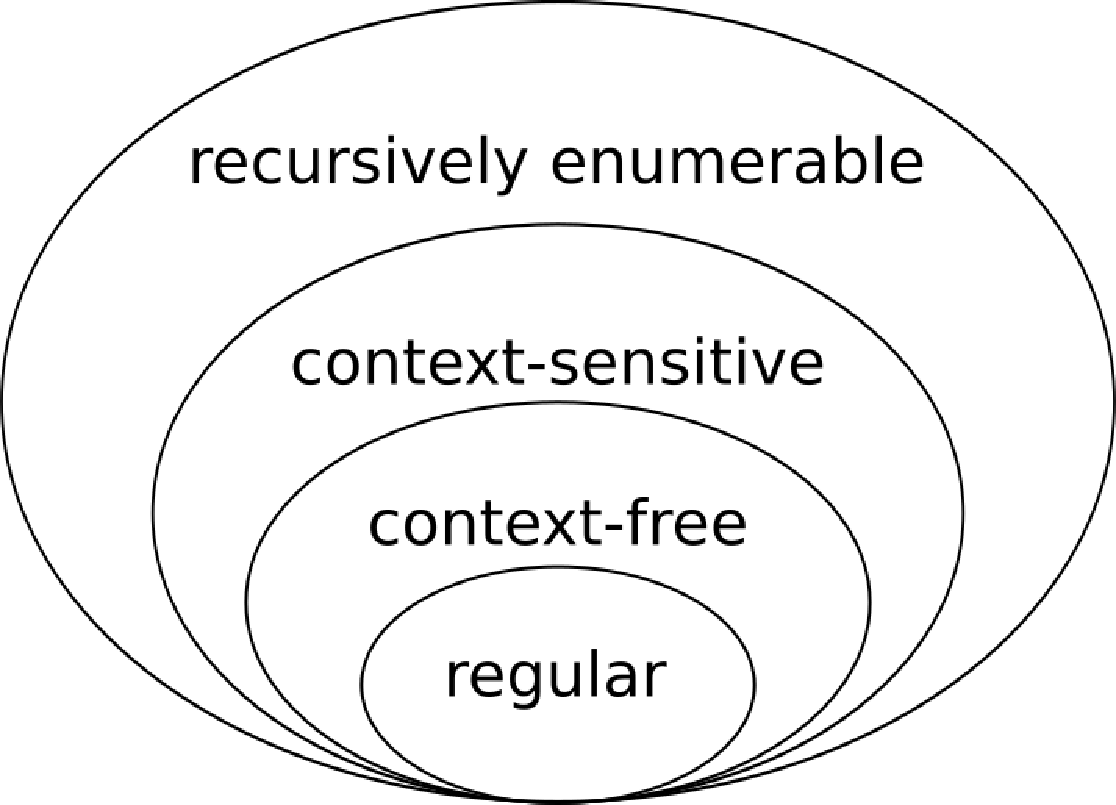
\includegraphics[height=.7\textheight]{Chomsky-hierarchy}
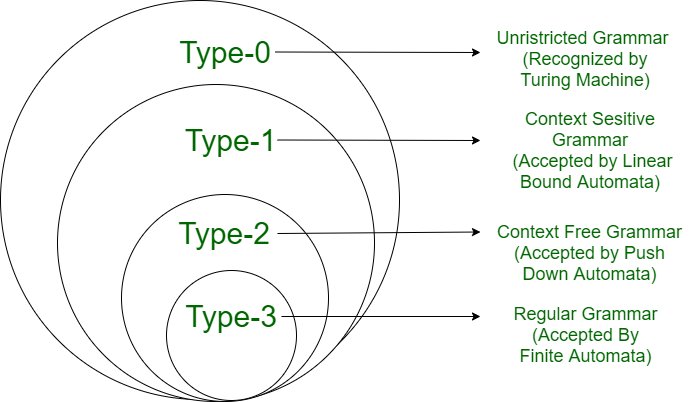
\includegraphics[height=.7\textheight]{Chomsky_types.png}

regular expressions are Type 3 whereas matching parenthesis require at least Type 2. 
\end{frame}

\section{Incompleteness, Turing machines and $\lambda$ calculus}
\begin{frame}
\frametitle{Church Turing Thesis/Conjecture}
Alonzo Church (PhD. adviser of Alan Turing):
"No computational procedure will be considered as an algorithm unless it can be represented as a Turing Machine"
\begin{center}
  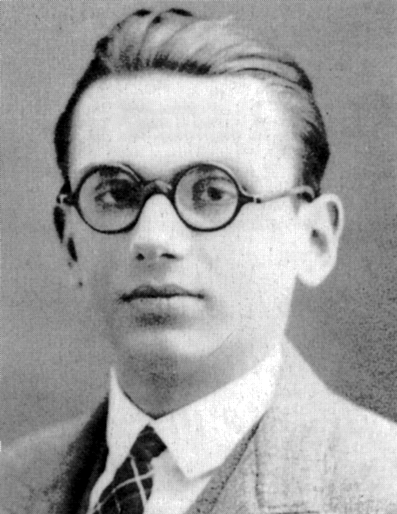
\includegraphics[height=.3\textheight]{1925_kurt_gödel.png}
  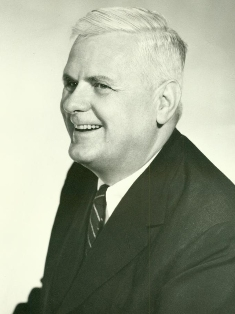
\includegraphics[height=.3\textheight]{Alonzo_Church.jpg}
  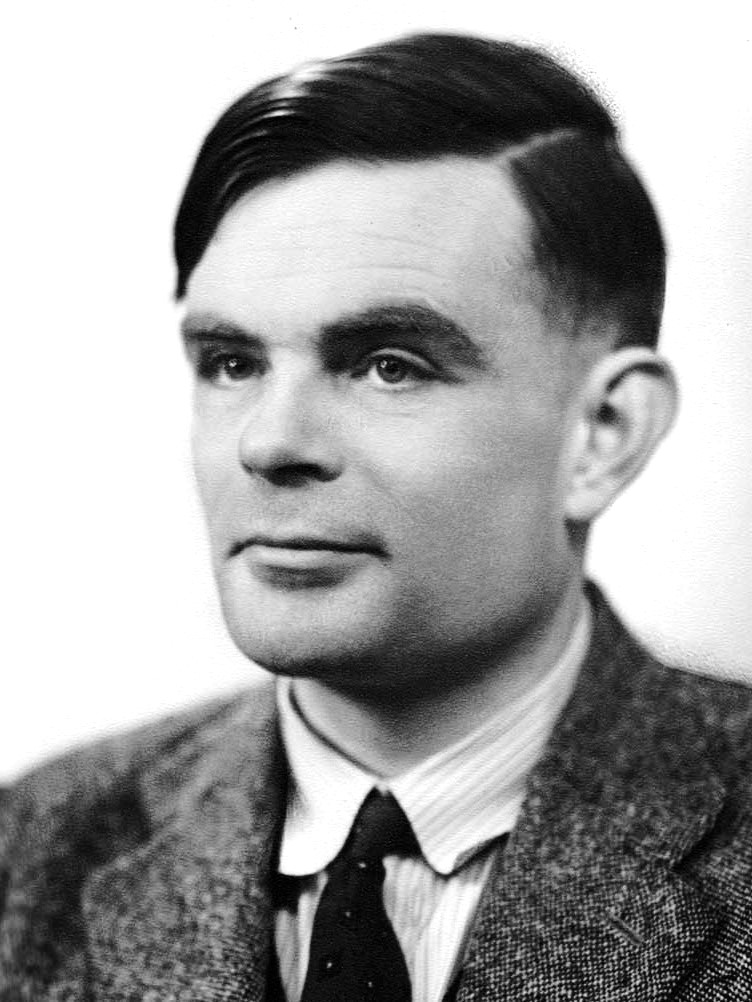
\includegraphics[height=.3\textheight]{Alan_turing.jpg}
  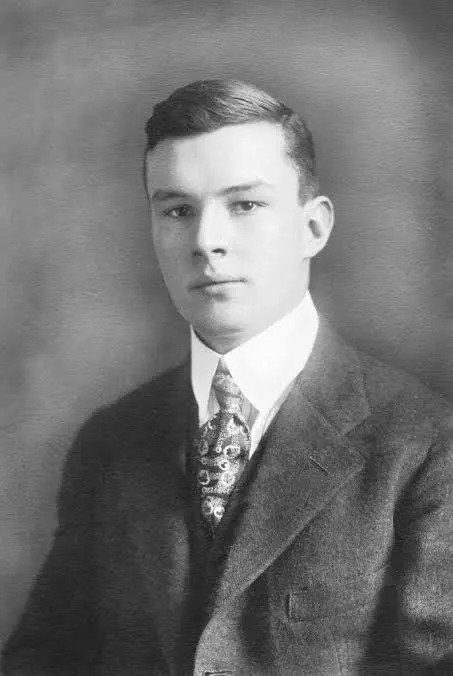
\includegraphics[height=.3\textheight]{HaskellCurry.jpg}
\end{center}
\end{frame}

\begin{frame}
\frametitle{Equivalence of Turing machines}
Fun facts:
\begin{itemize}
  \pause
    \item All modern programming languages are Turing complete (can simulate a Turing machine).
  \pause
    \item Even minimal languages (e.g. only a while loop) are Turing complete.
  \pause
    \item In particular the extremely minimal $\lambda$ calculus is. (proven not only according to the Church Turing Conjecture )\\
          e.g. in python: \texttt{lambda x: x**2}
  \pause
    \item As a corollary ``functional languages'' (which have no variables but only expressions) like Haskell, jax, or julia are. 
  \pause
\end{itemize}
Take home: According to Gödel not all things are computable, but the class of Computable problems is the same regardless of the definition (or language they are expressed in)
In particular: \alert{According to C.T it is worth trying to express any result that we can compute somehow  as a nested function call. }
\end{frame}

\begin{frame}
\frametitle{Referential transparency}

``... replacing a subexpression with another one that denotes the same value does not change the value of the expression.''
This is the basis for:
\begin{itemize}
\item memoization $\rightarrow$ caching by
\begin{itemize}
\item
  storing previos argument combinations the function was called with under a unique name
\item
  remembering the result of a function call by looking up combinations of arguments having occured before.
\end{itemize}
\item function transformation (derived properties like gradients) , compilation and automatic parallelization
\end{itemize}
\end{frame}


\section{Practical Problem description}

\begin{frame}
\frametitle{Many Models} 
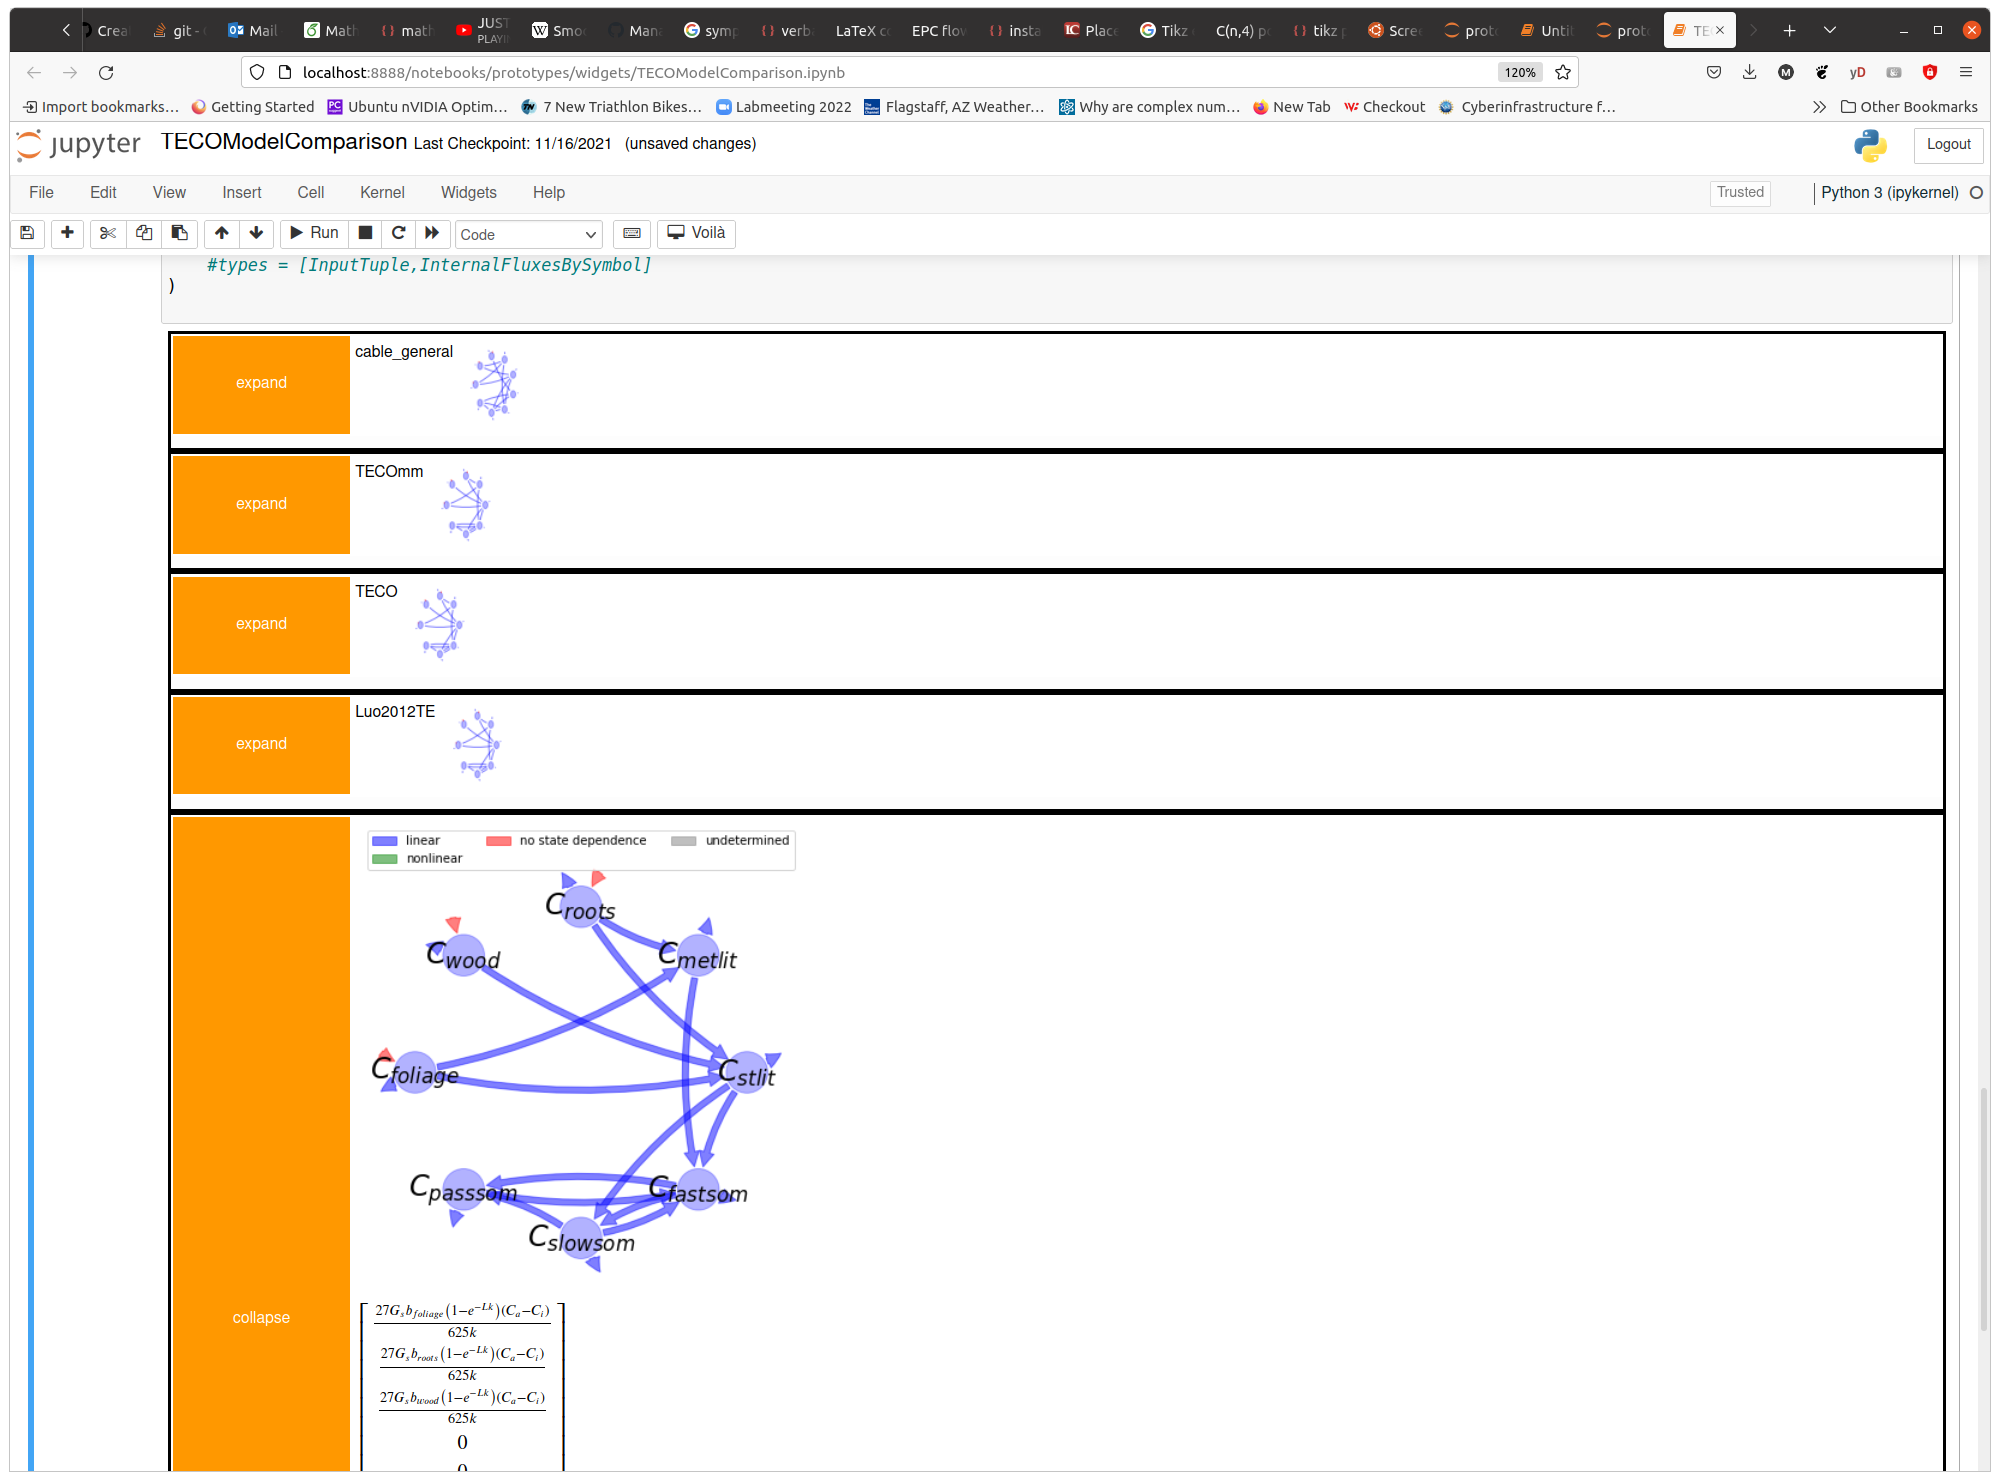
\includegraphics[height=.9\textheight]{ModelTable.png}
\end{frame}

\begin{frame}
\frametitle{ $Many^{Many} = \text{a lot}$} 
We want to estimate parameters for: 
\begin{itemize}
  \item
  different models  in 
  \item
  different variants for 
  \item
  different data sets with 
  \item
  different sampling algorithms based on 
  \item
  different ode solvers with 
  \item
  different parallelization strategies on 
  \item
  different hardware
\end{itemize}
and compare the results and the performance. 

\end{frame}

\begin{frame}
\frametitle{additional requirements:} 
\begin{itemize}
  \item
  Many computations occur in different comparisons. (caching becomes valuble)
  \item
  Some computations can only run on the cluster (caching should work over machine boundaries on file basis)
  \item
  Some collaborators have no access to our clusters but still need some of the results
  \item
  Some comparisons require query like filtering of results
\end{itemize}
\end{frame}

\begin{frame}
\frametitle{Implemented solution} 
\begin{itemize}
  \item Every job is described as a nested function call (A tree)..
  \item All leaves are basic data types so that the recursive call can be serialized as a json string (or automatically created python code)
  This makes it an extremely versatile (state less)  config file.

  \item The json string is hashable (e.g. sha256 or md5...but \alert{do not use pythons hash})
  \item The hash can be used to create a unique result directory also for branches of the tree 
  \item If the same task occures again the hash will be the same,  so will the result directory, so that compute intensive parts of the computation can be
  permanently memoized on disk.
\end{itemize}
\end{frame}

\begin{frame}
\frametitle{Implemented solution II} 
\begin{itemize}
  \item Since the job description can be serialized (written to a json file) it can be executed in different ways. 
  \begin{itemize}
    \item 
    Directly from python, 
    \item 
    indirectly in parallel subprocesses 
    \item 
    indirectly in automatically created 
    submission scripts on a cluster
  \end{itemize}
  \item Although not necessary the json config can also saved along side the cached results so that the result directory can be traversed and filtered like a 
  database. 
  \item The result directory (including all the hashed results) can be shared between computers (in our case a git subrepo since not all users have cluster access). The sha or md5 hashes are consistent over architectural boundaries the json files are human readable.
\end{itemize}
\end{frame}

\section{Functional Programming, random numbers and IO}
\begin{frame}
\frametitle{Some gotchas} 
  Not all functions in usual programming languages are functions in the mathematical sense (=\alert{pure} functions i.e. they do not always yield the same result if given the same arguments)
  \begin{itemize}
  \item obviously random number generators
  \item less obviously (=nasty) functions whose results are \alert{partially} randomized 
  e.g. \texttt{hash} in python is unique within one interpreter session (the next time you start python your cache id changes... 
  \item All functions that read files are at the mercy of the files not having changed by somebody else on disk...
  (That is the real reason why \alert{pure} functional languages like Haskell do not treat them as functions but put them in monadic containers.)
  $\rightarrow$ We have to take care ourselves that we do not violate our functional contract.
  \begin{itemize}
    \item The hash of our recursive function call will not change if we change the source code of one of the constituting functions even if that changes the functionality so that the results would change... In this case we would have to invalidate the cache ...
  \end{itemize}
  
  \end{itemize}
\end{frame}

\begin{frame}
\frametitle{Other benefits of a functional program description}
\note{
We use sampling algoriths that use the derivative of the mismatch of model and data with respect to the model parameters.
This is only possible because the functional framework (in this case jax can derive an expression for the gradient and compile it for different hardware architextures (cpus, gpus, tpus). This is another application of referential transparency)
}

  \begin{itemize}
    \item Automatic differentiation
    \item Automatic compilation for different hardware 
    \item Automatic parallelization (cpus, gpus, tpus)
  \end{itemize}
\end{frame}

\end{document}
